\chapter{Protocolli Automotive} %\label{1cap:spinta_laterale}
% [titolo ridotto se non ci dovesse stare] {titolo completo}
%

\begin{citazione}
In questo capitolo verranno illustrati i dettagli sui principali protocolli utilizzati nel mondo \emph{Automotive}, evidenziando punti di forza e debolezze. Successivamente, verrà effettuato un confronto tra questi in termini di prestazioni, applicabilità, costi, ecc.
\end{citazione}

\section{CAN}

\subsection{Caratteristiche del protocollo}
Il protocollo \emph{CAN} (Controller Area Network) è un protocollo basato su scambio di messaggi che permette a più dispositivi di trasmettere informazioni in maniera affidabile e in logica basata su \textbf{priorità}. Tutti i messaggi (o "\emph{frame}") inviati sono ricevuti da tutti i dispositivi connessi alla rete e, per questa ragione, la tipica topologia di rete usata in sinergia con \emph{CAN} è \textbf{BUS}, ovvero tutti i dispositivi appartenenti alla rete vengono collegati su un singolo cavo detto anche \emph{backbone}. Inoltre, è un protocollo \textbf{multi-master} \cite{huang_2019_invehicle}, in quanto non ha bisogno di un nodo master che fa da arbitro per l'intera rete ma tutti i nodi connessi sono in grado di comunicare autogestendosi, utilizzando come schema di arbitraggio \textbf{CSMA/CD} (Carrier-Sense Multiple Access with Collision Detection) \cite{can_notes}. Con questo schema, un dispositivo che vuole trasmettere un messaggio si mette prima in ascolto sul cavo e, se non rileva trasmissioni in corso, comincia a trasmettere il messaggio ascoltando quello che sta inviando. Se nel mentre che sta inviando il messaggio rileva un'interferenza, generata dall'arrivo di un altro messaggio già in fase di trasmissione, ferma immediatamente la trasmissione, trasmette una sequenza di \textbf{jamming} con lo scopo di avvertire gli altri dispositivi che è avvenuta una collisione e attende un tempo casuale prima di ritrasmettere (ovviamente dopo aver stabilito che il canale è libero) \cite{wikipedia_csmacd}. Uno schema per comprendere meglio il funzionamento dell'algoritmo \textbf{CSMA/CD} è mostrato nella \autoref{fig:csmacd-scheme}.
\begin{figure}[h]
    \centering
    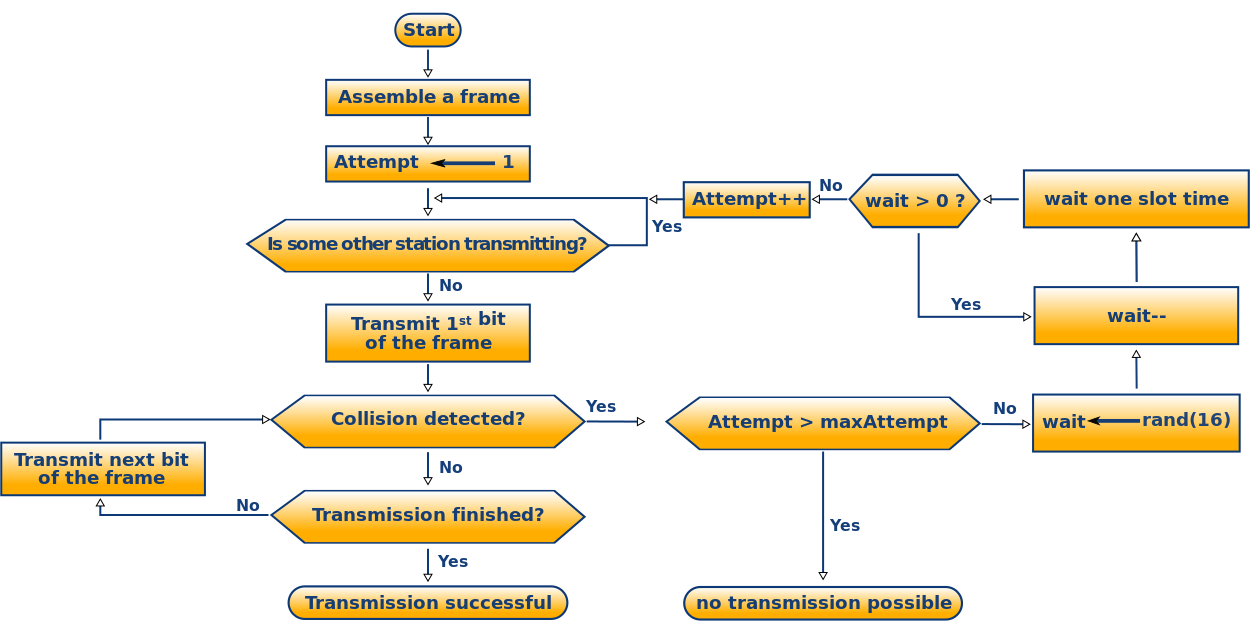
\includegraphics[width=0.7\textwidth]{capitoli/figure-protocolli/CSMACD-Algorithm.png}
    \caption{Diagramma di flusso di un algoritmo \textbf{CSMA/CD} con ritrasmissione}
    \label{fig:csmacd-scheme}
\end{figure}

Ogni dispositivo connesso alla rete viene chiamato \textbf{nodo} e deve essere composto almeno da una \emph{CPU} (processore per far funzionare tutto il dispositivo), un controller \emph{CAN} (componente che sappia parlare il protocollo \emph{CAN}) e un \emph{ricetrasmettitore} (componente che "legge e scrive" sui cavi elettrici).\\
È il protocollo più utilizzato in ambito \emph{Automotive} in quanto il suo utilizzo ha i seguenti vantaggi:

\begin{itemize}
    \item È un protocollo che richiede un cablaggio semplicissimo e poco costoso (un semplice cavo con due fili), riducendo la latenza, il peso della rete (in termini di kilogrammi), il numero di cavi necessari e il numero di errori;
    \item È completamente centralizzato e, per questa ragione, basta un qualunque punto di aggancio alla rete per accedere a tutto il traffico in circolazione e comunicare con tutte le \emph{ECU} connesse. Questo semplifica di molto il logging delle informazioni per fini diagnostici e la configurazione delle centraline;
    \item È molto robusto contro interferenze elettromagnetiche e disturbi elettrici, rendendolo ideale per applicazioni \textbf{safety-critical};
    \item Grazie all'integrazione di una logica basata su \textbf{priorità}, messaggi con \emph{ID} associati ad una priorità alta sono i primi ad accedere alla rete, senza causare interruzioni agli altri messaggi;
    \item Eliminando kilometri di cavi elettrici in eccesso, permette di ridurre il peso totale dell'automobile su cui è installata la rete migliorando anche i consumi di carburante;
    \item Dal momento che i chip e la strumentazione necessaria è molto semplice ed economica, abbassando di molto il costo necessario alla creazione della rete e delle \emph{ECU};
    \item Prevede meccanismi di correzione e rilevazione degli errori molto efficaci, permettendo alle informazioni di arrivare integre a destinazione;
    \item È facile aggiungere o rimuovere nodi dalla rete. \cite{can_bus_dewesoft}
\end{itemize}

\begin{figure}[h]
    \begin{subfigure}{0.45\textwidth}
        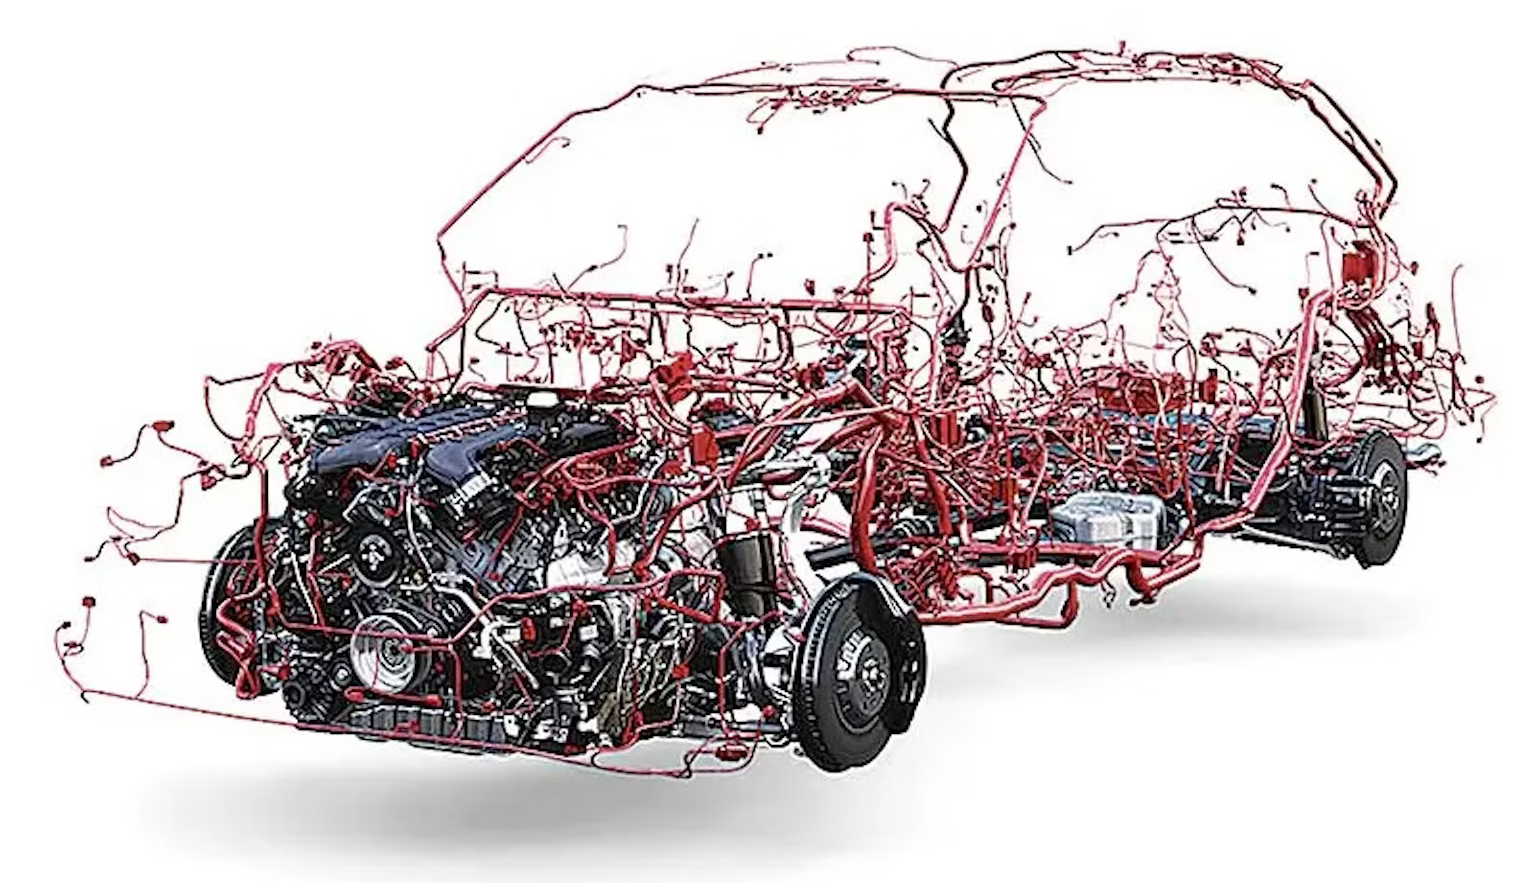
\includegraphics[width=1\textwidth]{capitoli/figure-protocolli/electrical-wiring-no-can.png}
        \caption{Cablaggio tipico di un'automobile che \textbf{NON} utilizza \emph{CAN}}
        \label{fig:electrical-wiring-no-can}
    \end{subfigure}
    \hfill
    \begin{subfigure}{0.45\textwidth}
        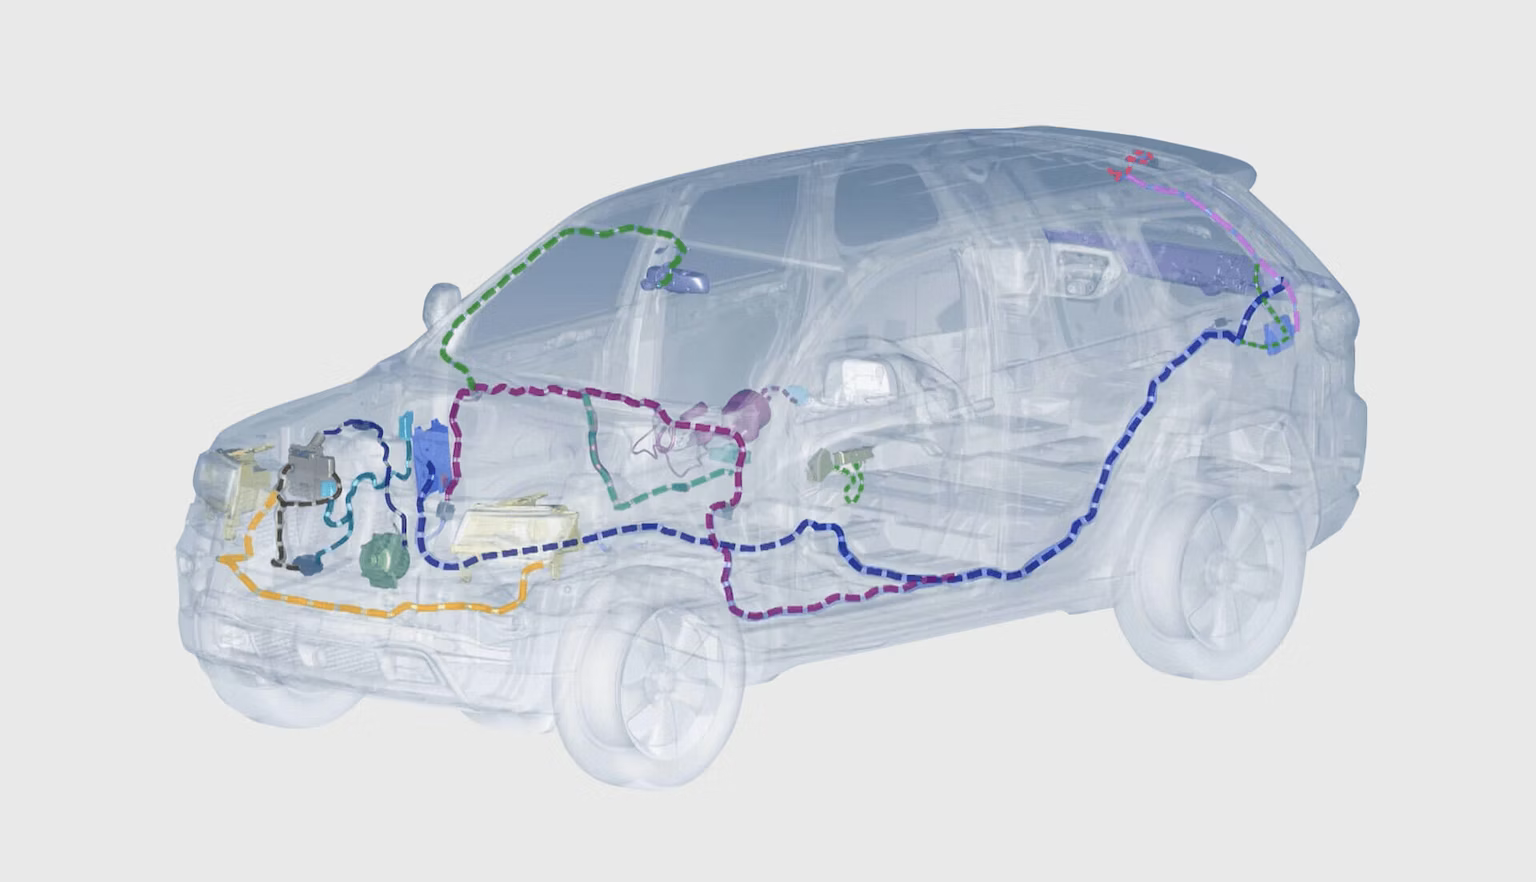
\includegraphics[width=1\textwidth]{capitoli/figure-protocolli/electrical-wiring-can.png}
        \caption{Cablaggio tipico di un'automobile che utilizza \emph{CAN}}
        \label{fig:electrical-wiring-can}
    \end{subfigure}
    \caption{Differenza di cablaggi con e senza \emph{CAN}}
    \label{fig:electrical-wiring-differences}
\end{figure}

Per via dei motivi sopracitati, oltre ad essere il protocollo più utilizzato in campo \emph{Automotive} è anche utilizzato in moltissimi altri ambiti, tra cui:

\begin{itemize}
    \item Aeronautica;
    \item Ascensori ed elevatori;
    \item Industrie e fabbriche;
    \item Navi;
    \item Elettrodomestici casalinghi come lavatrici, asciugatrici, ecc. \cite{can_bus_dewesoft}
\end{itemize}

\subsection{Struttura dei messaggi}
Ogni messaggio \emph{CAN} ha una struttura ben definita ed è composto da \textbf{header}, \textbf{payload} e \textbf{trailer}. Inoltre, è possibile individuare due tipologie di messaggi che sono \textbf{standard} e \textbf{esteso}, la cui unica vera differenza sta nella presenza di un campo \emph{ID} aggiuntivo nel messaggio (quindi cambia solo la lunghezza complessiva del messaggio).

\begin{figure}[h]
    \centering
    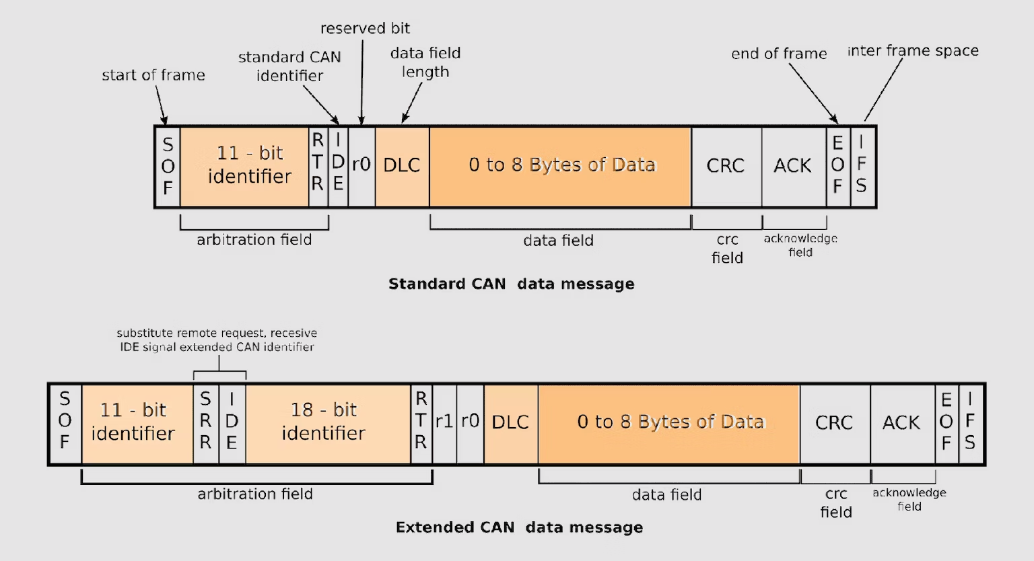
\includegraphics[width=0.7\textwidth]{capitoli/figure-protocolli/can-data-message-structure.png}
    \caption{Struttura dei messaggi \emph{CAN} \textbf{standard} ed \textbf{estesi}}
    \label{fig:can-message-structure}
\end{figure}

I vari campi di un tipico messaggio \emph{CAN} \textbf{standard} sono:
\begin{itemize}
    \item \textbf{SOF} (Start of Frame): 1 bit che indica l'inizio del messaggio e sincronizza i nodi dopo un periodo di inattività;
    \item \textbf{ID}: 11 bit che definiscono la priorità del messaggio, dove un identificativo più basso corrisponde ad una priorità più alta;
    \item \textbf{RTR}: 1 bit che viene impostato a $0$ (o \emph{dominante}) quando quello che si sta inviando è una \textbf{richiesta di informazione} (non un'informazione) e $1$ (o \emph{recessivo}) in caso contrario. Quando il bit viene impostato a $0$, non viene inviato nessun dato e l'\textbf{ID} determina l'informazione richiesta (quindi il nodo \emph{target});
    \item \textbf{IDE} (Identifier Extension): 1 bit che determina se il pacchetto è standard ($0$) o esteso ($1$);
    \item \textbf{r0}: 1 bit riservato che è privo di significato e lasciato per eventuali sviluppi futuri. Di solito è lasciato a $0$, ma anche se impostato a $1$ non fa differenza e viene accettato lo stesso;
    \item \textbf{DLC} (Data Length Code): 4 bit che indicano la lunghezza in \textbf{byte} del payload che contiene il messaggio;
    \item \textbf{Data}: 64 bit che indicano il dato che si sta inviando con il messaggio;
    \item \textbf{CRC} (Cyclic Redundancy Check): 16 bit che indicano il \textbf{checksum}, ovvero una \emph{somma} associata al campo \textbf{data} che viene utlizzata, tramite particolari operazioni matematiche, per effettuare rilevamento degli errori;
    \item \textbf{ACK} (ACKnowledgment): 1 bit che determina se un messaggio è stato ricevuto con successo ($0$) oppure sono stati rilevati degli errori ($1$). Chi invia il messaggio imposta il bit a $1$, metre chi riceve con successo imposta il bit a $0$;
    \item \textbf{EOF} (End of Frame): 7 bit che denotano la fine di un messaggio \emph{CAN}.
    \item \textbf{IFS} (Inter Frame Space): 3 bit recessivi (impostati a $1$) che separano il messaggio appena trasmesso da un nuovo messaggio. Dopo i primi 3 bit a $1$, il primo bit dominante (impostato a $0$) rilevato corrisponderà ad un bit \textbf{SOF}. \cite{can_bus_dewesoft} \cite{wikipedia_canbus}
\end{itemize}

Oltre ai campi di un messaggio \emph{standard}, i campi aggiuntivi in un messaggio \textbf{esteso} sono i seguenti:
\begin{itemize}
    \item \textbf{SRR} (Substitute Remote Request): 1 bit impostato a $1$ che serve a far prevalere sempre i messaggi \emph{standard} durante l'arbitraggio;
    \item \textbf{ID}: 18 bit che si aggiungono al primo campo \textbf{ID}, componendo un identificativo di 29 bit totali;
    \item \textbf{R1}: 1 bit riservato come \textbf{R0}, quindi anche in questo caso il valore associato a questo campo non ha significato e viene accettato qualunque sia.
\end{itemize}

Un'altra piccola differenza è che il campo \textbf{IDE} è posizionato prima del bit \textbf{RTR} e, in mezzo a questi due campi è posizionato il secondo campo \textbf{ID}.

\subsection{\emph{Bit stuffing}}
Per inviare i dati, a livello fisico, \emph{CAN} utilizza una codifica chiamata \textbf{NRZ} (Non-Return-to-Zero), ovvero il bit $1$ è codificato con un un voltaggio \emph{alto} mentre il bit $0$ con un voltaggio \emph{basso} e per codificare $n$ bit consecutivi basta inviare $n$ segnali \emph{alti} o \emph{bassi} in base al bit che si vuole inviare. Inoltre, la codifica può essere utilizzata secondo due tipologie:
\begin{itemize}
    \item \textbf{Unipolare}: il segnale \emph{alto} (quindi il bit $1$) è identificato da una differenza di voltaggio \textbf{positiva} (detto anche \emph{bias}), mentre il segnale \emph{basso} è identificato dall'assenza di un \emph{bias};
    \item \textbf{Bipolare}: il bit $1$ è codificato da un \emph{bias} positivo mentre il bit $0$ da un \emph{bias} negativo.
\end{itemize}

Esiste anche una codifica che fa da controparte, chiamata \textbf{RZ} (Return-to-Zero), nella quale un bit è identificato da una variazione di voltaggio seguito dal ritorno al valore \emph{normale} (nel caso dell'unipolare, il bit $0$ è identificato semplicemente dall'assenza di \emph{bias}). Una differenza tra le due codifiche (in versione unipolare) è mostrata in \autoref{fig:nrz-vs-rz}.
\begin{figure}[h]
    \centering
    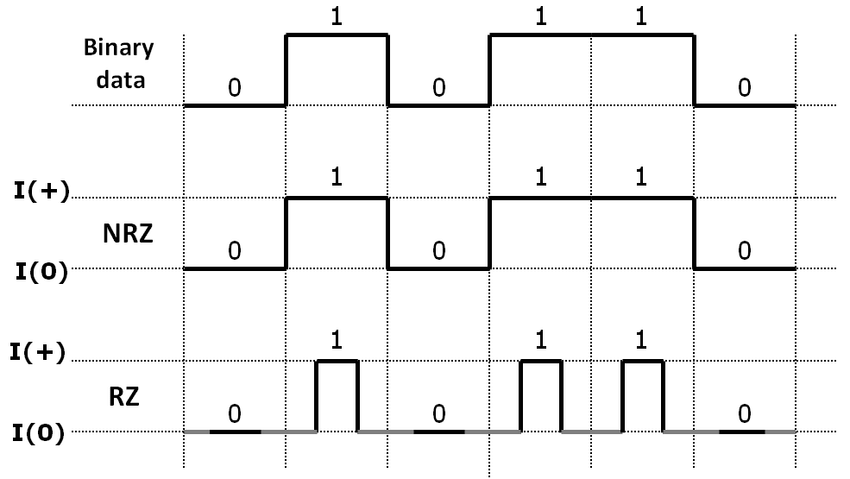
\includegraphics[width=0.5\textwidth]{capitoli/figure-protocolli/nrz-vs-rz.png}
    \caption{Differenza tra codifica \textbf{NRZ} e \textbf{RZ}, entrambe unipolari}
    \label{fig:nrz-vs-rz}
\end{figure}

Osservando le due codifiche, per inviare due bit $1$ con \textbf{NRZ} basta inviare due impulsi consecutivi alti, mentre con \textbf{RZ} bisogna inviare un impulso \emph{alto} seguito da un'assenza di \emph{bias} e, di nuovo un impulso \emph{alto} seguito da un'assenza di \emph{bias}. \cite{wikipedia_nrz}\\
Per via della natura della codifica \textbf{NRZ}, durante l'invio di molti bit consecutivi uguali c'è il rischio che i nodi perdano la sincronia e non siano più in grado di distinguere correttamente i bit inviati, questo poichè la polarità non varia per lunghi periodi di tempo. A questo proposito, l'invio dei messaggi con questa codifica viene affiancato da una tecnica chiamata \textbf{bit stuffing}, ovvero dopo l'invio di una certa soglia di bit uguali consecutivi viene inviato un bit di polarità inversa che non ha significato nel messaggio ma serve solo a mantenere i nodi sincronizzati (il bit viene detto \emph{di stuffing}). Ad esempio, immaginando che la soglia di bit consecutivi sia 4, se un nodo deve inviare la sequenza $111111$ (sei bit $1$ consecutivi), invierà la sequenza $1111011$ (dopo 4 bit invierà un bit \emph{di stuffing}). Ovviamente, il nodo che riceve il messaggio è a conoscenza della tecnica, è in grado di rimuovere correttamente i bit \emph{di stuffing} senza compromettere l'integrità del messaggio e nel momento in cui riceve un numero di bit consecutivi uguali al di sopra della soglia prestabilita rileva una violazione della codifica (nel caso di \emph{CAN} dopo ogni 5 bit uguali consecutivi, \textbf{DEVE} essere inviato un bit \emph{di stuffing}).

\subsection{Tipologie di messaggi}
Il protocollo \emph{CAN} prevede quattro tipologie di messaggi (o \emph{frame}), che si distinguono in base al compito che devono svolgere.
\subsubsection{Data Frames}
Questa tipologia di frame è l'unica che prevede l'utilizzo del campo \textbf{Data} e un \textbf{DLC} diverso da 0. È, quindi, la tipologia di messaggio che un nodo invia per condividere informazioni con uno o più nodi, associando all'identificativo il tipo di dato inviato e la priorità.

\subsubsection{Remote Frames}
Questa tipologia di frame permette ad un nodo di richiedere una specifica informazione, identificata dal campo \textbf{ID}. Anche se di solito le \emph{ECU} inviano le informazioni sulla rete di propria iniziativa quando l'informazione è pronta, a volte un nodo destinazione può richiedere uno specifico dato da uno specifico nodo. Questa tipologia di messaggio ha un payload vuoto in quanto non vuole inviare informazioni ma, tuttavia, il campo \textbf{DLC} è diverso da zero ed indica la lunghezza del dato \textbf{richiesto} e non "\textbf{inviato}". Infine, il campo \textbf{RTR} in questo caso è posto a $1$ (a differenza dei \emph{data frame}) in modo da associare una priorità più bassa a questa tipologia di messaggio e fargli perdere l'arbitraggio in caso di contesa con un \emph{data frame}. \cite{wikipedia_canbus}.

\subsubsection{Error Frames}
Questa tipologia di frame permette ai nodi, come espone in maniera molto chiara il nome, di segnalare eventuali errori rilevati a tutta la rete. La struttura di questi frame non segue quella descritta in precedenza ma è composta solo da 2 parti:
\begin{itemize}
    \item \textbf{Error flags}: tra 6 e 12 bit tutti \emph{dominanti} o tutti \emph{recessivi}, ottenuti dalla sovrapposizione di \emph{error frame} generati da nodi diversi;
    \item \textbf{Error Delimiter}: 8 bit tutti \emph{recessivi} che delimitano il frame.
\end{itemize}

La caratteristica fondamentale che contraddistingue questa tipologia di frame è il fatto che il campo \textbf{Error flags} è composto da bit uguali e non presenta bit \emph{di stuffing}, realizzando una violazione della regola del \emph{bit stuffing}.
Inoltre, ci sono due tipolgie di questi frame:
\begin{itemize}
    \item \textbf{Attivo}: tutti i bit del campo \textbf{Error flags} sono \emph{dominanti} e questo tipo di frame è generato da un nodo in modalità \textbf{attiva}, ovvero un nodo che per primo ha rilevato un errore;
    \item \textbf{Passivo}: tutti i bit del campo \textbf{Error flags} sono \emph{recessivi} e questo tipo di frame è generato da un nodo che è passato dallo stato \textbf{attivo} allo stato \textbf{passivo}.
\end{itemize}

Come già accennato, la tipologia di frame generato dipende dalla modalità in cui si trova il nodo, che può essere:
\begin{itemize}
    \item \textbf{Attiva}: modalità di default di ogni nodo. In questa modalità il nodo è in grado di inviare dati e frame di errore \textbf{attivi};
    \item \textbf{Passiva}: modalità in cui entrano i nodi che hanno generato un determinato numero di errori. In questa modalità i nodi sono in grado di inviare frame di errore \textbf{passivi} e sono in grado di inviare anche dati, tuttavia con l'obbligo di attendere 8 bit di \textbf{IFS} (invece dei classici 3 bit) prima di poter prendere il controllo della rete, in modo da dare la precedenza ai nodi \textbf{attivi};
    \item \textbf{Bus off}: modalità in cui entrano i nodi particolarmente \emph{problematici}. In questa modalità il nodo si disconnette completamente dalla rete e non è più in grado di inviare o ricevere messaggi.
\end{itemize}
Grazie a questo sistema, ai nodi \emph{problematici} verrà assegnata un livello di privilegio sempre più basso fino a spegnerlo del tutto nel caso in cui arrechi troppo disturbo alla rete.

Le varie transizioni tra le possibili modalità sono illustrate nella \autoref{fig:can-error-states}.
\begin{figure}[h]
    \centering
    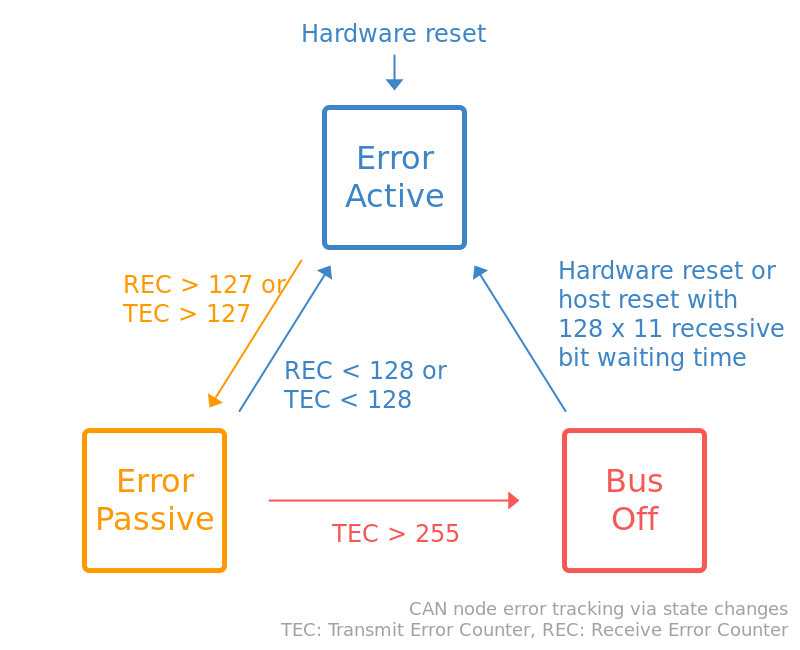
\includegraphics[width=0.6\textwidth]{capitoli/figure-protocolli/CAN-error-states.png}
    \caption{Modalità operative con relative transizioni}
    \label{fig:can-error-states}
\end{figure}

Per tenere traccia della modalità in cui si trova un nodo, vengono impiegati due registri:
\begin{itemize}
    \item \textbf{TEC} (Transmit Error Counter);
    \item \textbf{REC} (Receive Error Counter).
\end{itemize}
L'utilizzo di questi due registri permette ad un nodo di capire come si sta comportando e, in base al valore raggiunto da questi, cambierà modalità e si comporterà come stabilito. I valori dei due registri vengono aggiornati come illustrato nella \autoref{fig:can-error-counter} e, inoltre, nella \autoref{fig:can-error-types} sono illustrati i possibili errori che un nodo può rilevare. \cite{css_electronics_can} \cite{wikipedia_canbus}
\begin{figure}[h]
    \begin{subfigure}{0.45\textwidth}
        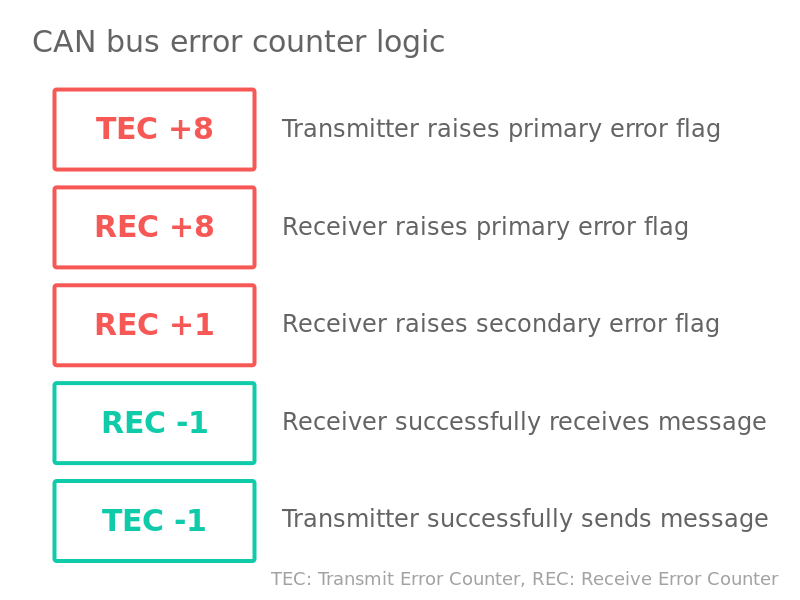
\includegraphics[width=1\textwidth]{capitoli/figure-protocolli/CAN-bus-error-counter.png}
        \caption{Variazioni dei registri di errore}
        \label{fig:can-error-counter}    
    \end{subfigure}
    \hfill
    \begin{subfigure}{0.45\textwidth}
        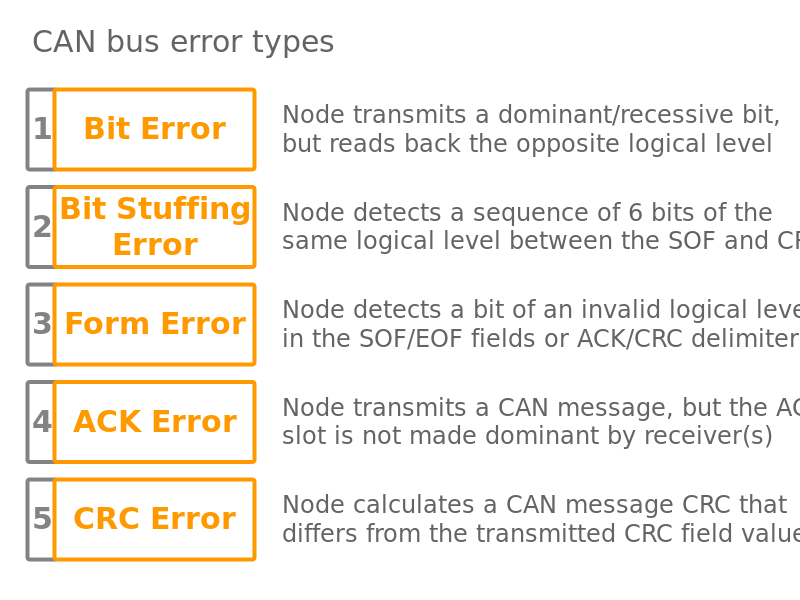
\includegraphics[width=1\textwidth]{capitoli/figure-protocolli/CAN-bus-error-types.png}
        \caption{Errori possibili in \emph{CAN}}
        \label{fig:can-error-types}
    \end{subfigure}
    \caption{Rilevazione e gestione degli errori in \emph{CAN}}
    \label{fig:can-error}
\end{figure}


\subsubsection{Overload Frames}
Questa tipologia di frame permette ad un nodo saturo di avvisare gli altri nodi di fermare la trasmissione di frame di \textbf{dati} e \textbf{remoti}. La struttura è uguale ai frame di \textbf{errore} ma la differenza sta nel momento in cui viene inviato, ovvero durante la trasmissione dell'\textbf{IFS}. \cite{wikipedia_canbus}

\subsection{Varianti del protocollo}
Esistono alcune varianti del protocollo \emph{CAN}, con lo scopo di adattarlo ad ambienti e requisiti diversi. Sebbene se ne possano trovare diverse in letteratura, le principali varianti sono tre.

\subsubsection{Low Speed CAN}
Variante del protocollo con velocità di trasmissione massima di circa 125 Kbps, utilizzata in sistemi con elevati requisiti di affidabilità, che non richiedono una larghezza di banda elevata e che non richiedono aggiornamenti molto frequenti. Il cablaggio richiesto è molto più economico e di solito viene utilizzato in sitemi diagnostici, nei controlli e display del cruscotto, ecc. \cite{can_bus_dewesoft}

\subsubsection{High Speed CAN}
Variante del protocollo con velocità di trasmissione massima di circa 1 Mbps, utilizzata in sistemi che richiedono aggiornamenti molto più frequenti ed un'elevata precisione. Richiede un cablaggio più costoso rispetto alla variante \textbf{Low Speed} ma permette il corretto funzionamento di sistemi \emph{safety-critical} come \textbf{ABS}, airbag, controllo della stabilità, controlli del motore, ecc. \cite{can_bus_dewesoft}

\subsubsection{CAN FD}
Variante del protocollo (chiamata "\emph{CAN} sotto steroidi" \cite{can_bus_dewesoft}) con velocità di trasmissione in grado di raggiungere circa 5 Mbps. Per raggiungere queste velocità si contraddistingue dalle due varianti precedenti sulla lunghezza del payload, dove prima poteva avere una lunghezza massima di 8 Byte mentre con \emph{CAN FD} (Flexible Data-Rate) si possono raggiungere i 64 Byte (incremento dell'800\%). Per realizzare questo incremento, ovviamente, l'header è leggermente diverso da quello standard ma è stato realizzato in modo da essere retrocompatibile con le trasmissioni \emph{CAN} standard.

Le modifiche rispetto ad un frame standard sono:
\begin{itemize}
    \item \textbf{RSS} (Remote Request Substitution) vs \textbf{RTR}: essendo che in \emph{CAN FD} non esistono messaggi \textbf{remoti}, il bit \textbf{RTR} è sostituito con \textbf{RSS} ed è sempre $0$; 
    \item \textbf{FDF} (Flexible Data-Rate Format) vs \textbf{R0}: il bit riservato \textbf{R0} è sostituito con il bit \textbf{FDF} che è sempre $1$ e stabilisce che il messaggio è di tipo \emph{FD}. In questa tipologia di messaggio vengono introdotti anche tre bit aggiuntivi;
    \item \textbf{RES}: 1 bit riservato per sviluppi futuri per cui il suo valore non è influente. È aggiuntivo rispetto al frame standard;
    \item \textbf{BRS} (Bit Rate Switch): 1 bit che se impostato a $0$ indica che la velocità di trasmissione sarà quella della fase di arbitraggio (velocità fino a 1 Mbps) mentre se impostato a $1$ indica che verrà utilizzata una velocità superiore (fino a 5 Mbps). Anche questo è aggiuntivo rispetto al frame standard;
    \item \textbf{ESI} (Error Status Indication): 1 bit che indica la \emph{modalità} in cui è entrato il nodo, quindi sarà $0$ se il nodo è in modalità \textbf{attiva} mentre $0$ se il nodo è in modalità \textbf{passiva}. Anche questo nodo è aggiuntivo rispetto al frame standard;
    \item \textbf{DLC}: Come nei frame standard, anche qui indica la lunghezza del payload. Tuttavia, a differenza dello standard, la corrispondenza tra valore in bit e lunghezza è leggermente diversa per permettere l'invio di payload più lunghi di 8 byte (la mappatura è indicata in \autoref{fig:canfd-dlc});
    \item \textbf{SBC} (Stuff Bit Count): 3 bit che rispettano la codifica di Gray, seguiti da un bit di parità. Sono stati aggiunti per migliorare l'affidabilità della comunicazione;
    \item \textbf{CRC}: 17 bit o 21 bit per il controllo degli errori dei payload di 16 Byte o 20-64 Byte, rispettivamente. A differenza dei messaggi standard, nei messaggi \emph{CAN FD} sono impostati \textbf{SEMPRE} 4 bit di stuffing, mentre prima potevano essercene tra 0 e 3;
    \item \textbf{FSB} (Fixed Stuff Bit): bit di stuffing impostati prima e dopo \textbf{SBC} e all'interno del campo \textbf{CRC};
    \item \textbf{ACK}: questo campo delimita la fine dell'invio a velocità superiori, ritornando alla velocità di default di \emph{CAN}.
\end{itemize}

\begin{figure}[h]
    \begin{subfigure}{0.45\textwidth}
        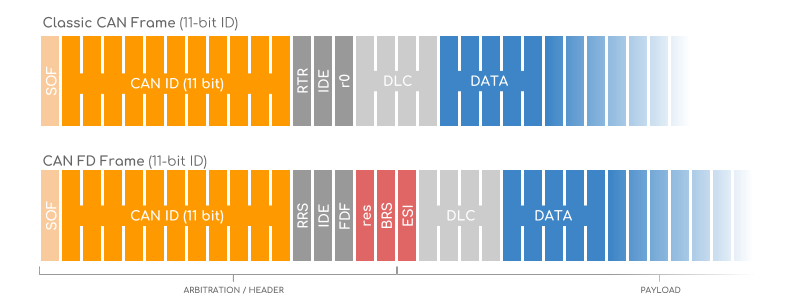
\includegraphics[width=1\textwidth]{capitoli/figure-protocolli/canfd-header.png}
        \caption{Header \emph{CAN FD} vs. header \emph{CAN}}
        \label{fig:canfd-header}
    \end{subfigure}
    \hfill
    \begin{subfigure}{0.45\textwidth}
        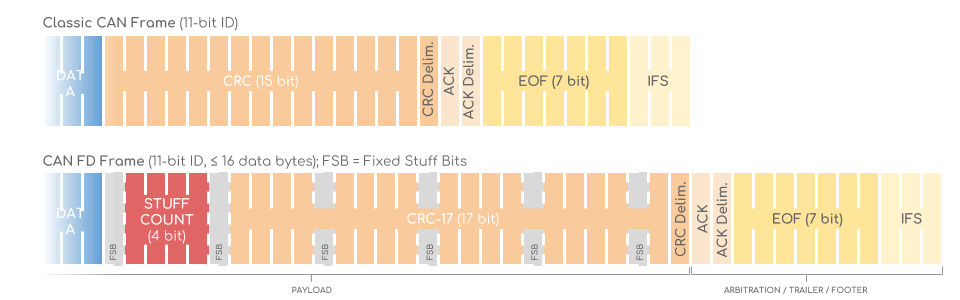
\includegraphics[width=1\textwidth]{capitoli/figure-protocolli/canfd-trailer.png}
        \caption{Trailer \emph{CAN FD} vs. trailer \emph{CAN}}
        \label{fig:canfd-trailer}
    \end{subfigure}
    \centering
    \begin{subfigure}{0.8\textwidth}
        \vspace{0.3cm}
        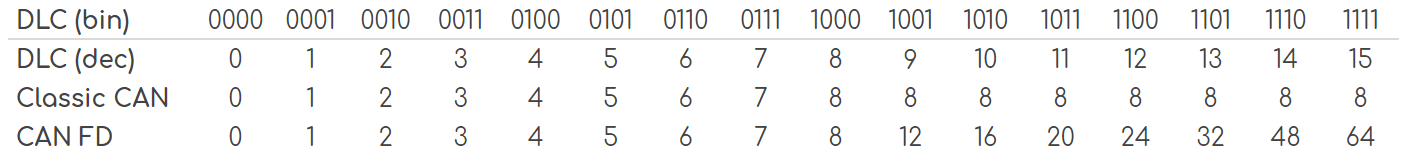
\includegraphics[width=1\textwidth]{capitoli/figure-protocolli/canfd-dlc.png}
        \caption{Mappatura dei valori di \textbf{DLC} in \emph{CAN FD} e \emph{CAN}}
        \label{fig:canfd-dlc}
    \end{subfigure}
    \caption{Differenze tra \emph{CAN FD} e \emph{CAN}}
    \label{fig:canfd-differences}
\end{figure}

Un altro vantaggio molto importante che introduce questa variante è la possibilità di variare in maniera adattiva la velocità di trasmissione dei messaggi. Questo permette ai nodi di adattarla in base a ciò che si vuole inviare, lasciando la velocità invariata o accelerando in caso di dati più urgenti o messaggi più lunghi.

Rispetto alla variante standard, con \emph{CAN FD} si possono realizzare sistemi più complessi che richiedono requisiti di banda più stringenti. Ad esempio, si possono realizzare sistemi \textbf{ADAS} (Advanced Driver Assistance System) come cruise control adattivo, frenata automatica d'emergenza, moonitoraggio degli angoli ciechi, ecc. \cite{css_electronics_canfd}

\section{FlexRay}
Con il procedere degli anni e con lo sviluppo di sistemi sempre più avanzati e complessi, è stato raggiunto un punto dove il protocollo \emph{CAN} comincia a far pesare i propri limiti. Se si pensa all'aumento del numero delle \emph{ECU} all'interno delle automobili, allo sviluppo di sistemi \textbf{X-\emph{by-wire}} e all'implementazione di sistemi di sicurezza sempre più all'avanguardia, anche utilizzando la variante \emph{CAN FD} non si riescono a garantire i sempre più stringenti requisiti di banda e di affidabilità richiesti per il corretto funzionamento di tutti i sistemi. È proprio per questo motivo che un team specializzato ha realizzato \textbf{FlexRay}, un protocollo in grado di soddisfare elevati requisiti di banda, sicurezza, affidabilità e velocità di trasmissione. Non nasce con l'idea di sostituire \emph{CAN} ma, piuttosto, con quella di affiancarsi e cooperare con esso, sebbene la tendenza che stanno seguendo i produttori è di sostituire \emph{CAN} con \emph{FlexRay}.

\subsection{Caratteristiche del protocollo}
Il protocollo \emph{FlexRay} presenta diversi vantaggi:
\begin{itemize}
    \item Permette il raggiungimento di una larghezza di banda di 10 Mbps, molto più alta rispetto a \emph{CAN} e permette di variare la velocità di trasmissione in base alle necessità;
    \item Richiede un cablaggio semplice, composto da un cavo con due o quattro fili \cite{ni_flexray}, ma è in grado di lavorare anche con cablaggi di tipo ottico;
    \item Supporta diverse topologie di rete oltre al \textbf{BUS};
    \item Assicura una maggiore tolleranza ai guasti maggiore e determinismo;
    \item Permette l'invio di payload fino ad una lunghezza massima di 254 Byte, circa 30 volte più grande di \emph{CAN};
    \item Consente l'accensione e lo spegnimento dei nodi in maniera dinamica per permettere una riduzione dei consumi elettrici.
\end{itemize}

\subsubsection{Costi}
Sebbene sia migliore di \emph{CAN} sotto molti aspetti, lo svantaggio più importante è il costo rischiesto per una rete \emph{FlexRay}, in quanto richiede cavi più costosi per garantire una banda più alta e dispositivi più sofisticati. Tuttavia, essendo che il protocollo è stato realizzato in maniera da poter cooperare con \emph{CAN} e altri protocolli, è possibile abbattere i costi di produzione utilizzando \emph{FlexRay} solo dove strettamente necessario, quindi per sistemi avanzati con stringenti requisiti di affidabilità e banda, e dove non è necessario si può utilizzare \emph{CAN} o altri protocolli che richiedono cablaggi più economici. \cite{eos_flexray}

\subsubsection{Affidabilità}
Per una migliore tolleranza ai guasti, \emph{FlexRay} utilizza i due fili come due canali di comunicazione separati, infatti, una \emph{ECU} che opera con questo protocollo ha bisogno di un \textbf{controllore FlexRay} che permette l'utilizzo del protocollo stesso e due \textbf{ricetrasmettitori} che permettono di "scrivere" e "leggere" su entrambi i fili in maniera indipendente (come mostrato in \autoref{fig:flexray-node-structure}) e inviare uno stesso messaggio in maniera ridondata su entrambi i fili (oppure una sola volta su uno solo filo in base alla configurazione). I due fili possono essere usati anche come canali separati per inviare messaggi diversi, aumentando in questo modo la larghezza di banda disponibile. Inoltre, \emph{FlexRay} utilizza anche un ulteriore circuito (opzionale), chiamato \textbf{Bus Guardian} \cite{eos_flexray}, il cui scopo è quello di rilevare interferenze generate da messaggi non sincronizzati e proteggere il canale da questi. Utilizzando questo ulteriore dispositivo si riduce in maniera drastica la possibilità di ottenere collisioni. \cite{eos_flexray}

\begin{figure}[h]
    \centering
    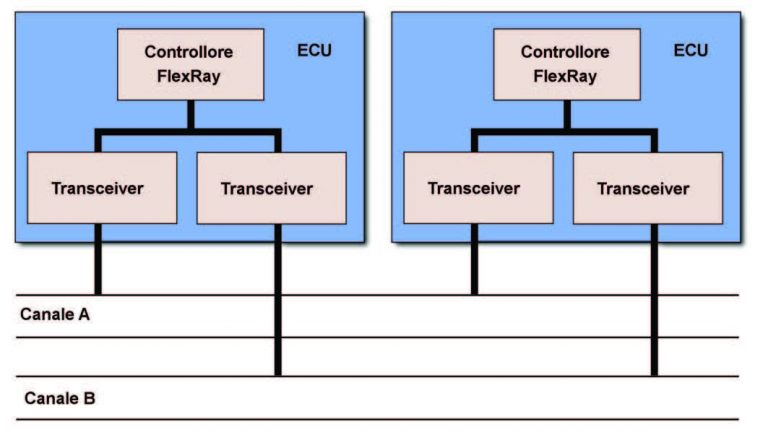
\includegraphics[width=0.7\textwidth]{capitoli/figure-protocolli/flexray-node-structure.jpg}
    \caption{Struttura tipica di una \emph{ECU} che utilizza \emph{FlexRay}}
    \label{fig:flexray-node-structure}
\end{figure}

\subsubsection{Determinismo}
\emph{FlexRay} utilizza un meccanismo di arbitraggio chiamato \textbf{TDMA} (Time Division Multiple Access), ovvero ad ogni nodo della rete viene assegnato uno \emph{slot} temporale in cui può trasmettere un messaggio. Affinchè non ci siano collisioni, è necessario che ogni nodo della rete abbia il proprio \emph{clock} sincronizzato con gli altri, altrimenti un nodo potrebbe trasmettere in uno slot che non gli è stato assegnato facendo collidere il proprio messaggio con quello inviato dal nodo \emph{legittimo}. Essendo un sistema distribuito, i nodi non hanno un clock fisico \textbf{assoluto} a cui far riferimento, ma vengono impiegati diversi \textbf{nodi di sincronizzazione}, il cui scopo è quello di inviare periodicamente \textbf{frame di sincronizzazione} che aiutino i nodi della rete ad aggiustare il proprio clock in caso di \emph{sfasature}. Così facendo, tutti i clock (compresi quelli dei nodi di sincronizzazione) rimangono allineati garantendo il corretto funzionamento dell'arbitraggio \textbf{TDMA}. \cite{eos_flexray}

\subsection{Ciclo di comunicazione}
In \emph{FlexRay} l'accesso al canale condiviso è basato sull'assegnamento di uno slot temporale ad ogni nodo, all'interno del quale è possibile inviare un messaggio. Questo assegnamento viene reiterato in un ciclo che prende il nome di \emph{ciclo di comunicazione} ed è l'elemento principale dello schema di accesso al canale condiviso. È definito in termini di una \textbf{gerarchia temporale} composta da 4 livelli, che sono i seguenti:
\begin{itemize}
    \item \textbf{Communication Cycle}: è il livello più alto e definisce il ciclo in termini di 4 fasi (o segmenti), che sono \textbf{segmento statico}, \textbf{segmento dinamico}, \textbf{symbol window} e \textbf{network idle time};
    \item \textbf{Arbitration Grid}: livello subito inferiore al precedente ed è lo scheletro di tutto lo schema di arbitraggio. Divide i vari segmenti in sezioni temporali che è possibile assegnare ai vari nodi della rete e, in particolare, nel \emph{segmento statico} queste sezioni prendono il nome di \textbf{slot statici} mentre nel \emph{segmento dinamico} prendono il nome di \textbf{minislot}. La differenza tra questi due sta nel meccanismo di arbitraggio utilizzato per assegnarli ai vari nodi. 
    \item \textbf{Macrotick}: livello subito inferiore al precedente e definisce la durata di un ciclo e di ogni segmento e sezione, i quali hanno una durata corrispondente ad un numero intero di \emph{Macrotick}. Un \emph{Macrotick} si definisce come \textbf{un numero intero di \emph{Microtick}};
    \item \textbf{Microtick}: livello più basso e definisce l'elemento base di tutto il ciclo, il \emph{Microtick}. Esso non è altro che un numero intero di \emph{tick} (ticchettii, battiti) del clock di un oscillatore presente in un \emph{controllore FlexRay} di un nodo (come in un normale processore all'interno di un computer).
\end{itemize}

\subsubsection{Segmento statico}

\begin{figure}[h]
    \centering
    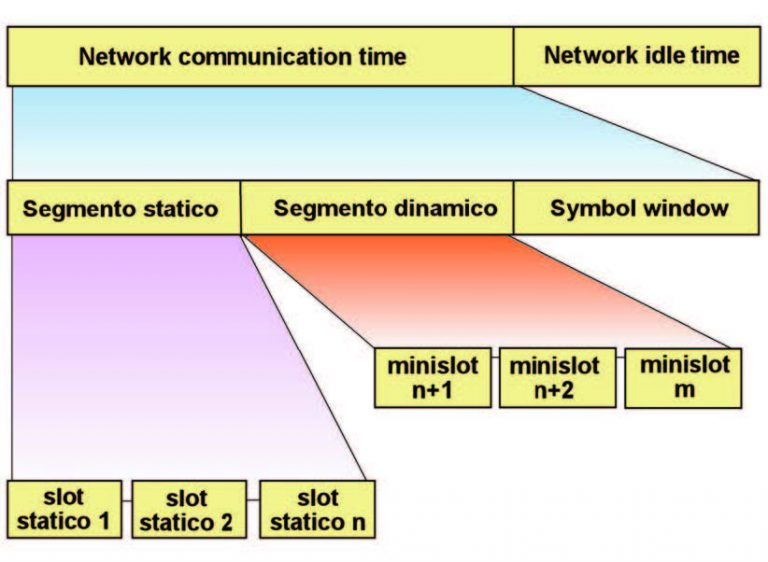
\includegraphics[width=0.6\textwidth]{capitoli/figure-protocolli/flexray-communication-cycle.jpg}
    \caption{Suddivisione del ciclo di comunicazione}
    \label{fig:communication-cycle-segments}
\end{figure}
Segmento sempre presente in ogni \emph{ciclo di comunicazione} ed è la fase iniziale del ciclo. Questa fase è suddivisa in \emph{slot statici} dalla stessa lunghezza in \textbf{Macrotick} e il numero dipende dalla configurazione della rete. Questi slot vengono assegnati in maniera statica ai nodi della rete e, quindi, il meccanismo di arbitraggio presente in questa fase è il \textbf{TDMA}. Affinchè tutti i nodi siano in grado di rispettare i turni, ognuno mantiene un \emph{contatore di slot} (uno per ogni canale) che viene incrementato ad ogni numero di \textbf{Macrotick} corrispondente alla lunghezza di uno \emph{slot statico}. In questo modo, tutti sono a conoscenza dello slot corrente e a chi è assegnato. \cite{flexray_specification}\\
Questa fase garantisce un livello di determinismo massimo, dal momento che tutti sanno quando gli altri trasmetteranno dati, tuttavia un \emph{segmento statico} troppo lungo rischia di rallentare inevitabilmente la rete e introdurre latenze eccessive per messaggi urgenti. Inoltre, se un nodo non invia nulla durante il proprio \emph{slot statico}, questo è interamente sprecato e bisogna attendere la fase successiva o il successivo ciclo. \cite{ni_flexray}

\subsubsection{Segmento dinamico}
Segmento successivo e opzionale a quello \emph{statico} che può essere omesso in fase di configurazione della rete. Questa fase è suddivisa in \emph{minislot} tipicamente lunghi pochi \textbf{Macrotick} (anche uno solo e, in generale, più breve di uno \emph{slot statico} \cite{eos_flexray}) e, anche qui, il numero di \emph{minislot} dipende dalla configurazione della rete. In questa fase, i \emph{minislot} vengono assegnati in base alla priorità delle informazioni da inviare, quindi un nodo che deve inviare un'informazione con priorità più elevata avrà assegnato un \emph{minislot} più vicino all'inizio della fase mentre un nodo con informazioni meno prioritarie avrà assegnato un \emph{minislot} più lontano. Anche in questa fase vengono impiegati dei contatori per stabilire in quale \emph{minislot} ci si trova, solo che a differenza del \emph{segmento statico} la durata di un singolo \emph{minislot} può variare:
\begin{itemize}
    \item Se il nodo a cui è assegnato il \emph{minislot} rimane in \emph{idle} e non trasmette nulla, la durata di questo effettivamente definito in fase di configurazione della rete;
    \item Se il nodo decide di trasmettere, la durata del \emph{minislot} viene "\emph{espansa}" facendolo durare più \emph{minislot} e permettendo la trasmissione dell'intero dato senza interruzioni e in maniera \emph{fault-tolerant}.
\end{itemize}

Questo schema di "espansione" permette di non perdere larghezza di banda preziosa nel caso in cui uno o più nodi decidano di non inviare nulla. Inoltre, è necessario perchè la durata di un \emph{minislot} è tale da non riuscire ad includere un'intero messaggio \emph{FlexRay} e, per questa ragione, quando un nodo decide di trasmettere ha bisogno di un intervallo più lungo.\\
Come già anticipato, anche qui vengono utilizzati dei contatori per tenere traccia del \emph{minislot} in cui ci si trova ma, essendo che chi trasmette acquisisce più \emph{minislot}, viene fissato un limite di \emph{minislot} "effettivi" oltre il quale passare alla fase successiva (o ciclo successivo) anche se non si è raggiunto il numero di \emph{minislot} "definito". Questo significa che i nodi con messaggi meno prioritari potrebbero perdere il proprio turno e trasmettere nella fase successiva, ma non è un problema in quanto essendo meno prioritari sono meno suscettibili alle latenze rispetto a quelli con priorità più alta. \cite{eos_flexray} \cite{flexray_specification}\\
Lo schema di arbitraggio utilizzato in questa fase ricorda molto quello utilizzato da \emph{CAN}.

\subsubsection{Symbol Window}
Segmento successivo al \emph{dinamico} ed è una fase dove vengono scambiati messaggi di gestione della rete. Tipicamente le applicazioni di alto livello non interagiscono con questa fase \cite{ni_flexray} e i messaggi inviati possono essere di sincronizzazione del clock, di allarmi vari o di wakeup o startup. Anche la lunghezza di questa fase è definita in fase di configurazione e in termini di \textbf{Macrotick}.

\subsubsection{Network Idle Time}
Segmento successivo alla \emph{Symbol Window} ed è una fase in cui non avviene nessuno scambio di messaggi. Lo scopo di questa fase è quella di permettere ai nodi della rete di effettuare aggiustamenti al proprio clock interno per correggere eventuali \emph{drift} e di eseguire eventuali task aggiuntivi relativi al ciclo di comunicazione. Anche la durata di questa fase è definita in fase di configurazione e tipicamente è molto breve, questo perchè essendo un periodo di inattività tutta la banda assegnata a questa fase è sprecata. Il tutto risulta nell'introduzione di latenze aggiuntive che devono essere ottimizzate facendo durare questa fase il meno possibile. \cite{flexray_specification}

\subsection{Sincronizzazione del Clock}
In un sistema distribuito come una rete \emph{FlexRay}, ogni nodo ha il proprio \emph{clock} con cui scandisce il tempo. Tuttavia, a causa di fluttuazioni di temperatura, fluttuazioni di voltaggio, purità dei materiali usati nell'oscillatore, differenze dovute alla produzione, ecc. può succedere che i \emph{clock} scandiscano il tempo in maniera diversa (più o meno veloce) e questo significa che anche se i \emph{clock} partono sincronizzati, questi divergono dopo piccoli intervalli di tempo. In un sistema basato quasi interamente su turni e intervalli temporali, ovviamente, clock non affidabili portano all'impossibilità di comunicare senza errori e con le prestazioni desiderate. Per questa ragione, è necessario che un meccanismo di \textbf{sincronizzazione dei clock} che, a intervalli regolari, sincronizzi tutti i \emph{clock} prima che questi divergano compromettendo la rete. Non è necessario che questi siano \textbf{perfettamente} sincronizzati, piuttosto basta che ogni coppia di nodi indichi il "tempo globale" con una differenza che non supera una determinata soglia. \cite{flexray_specification}

Affinchè i nodi rimangano sincronizzati, \emph{FlexRay} prevede la presenza di \textbf{nodi di sincronizzazione} il cui scopo è quello di inviare dei messaggi chiamati \emph{sync frame} ad ogni ciclo che vengono utilizzati da tutti i nodi per correggere il proprio clock da eventuali \emph{drift} (deviazioni). Sebbene il numero di \textbf{Microtick} necessari per un \textbf{Macrotick} sia definito in fase di configurazione della rete, un nodo può modificare questo valore in maniera dinamica per correggere il \emph{drift} del proprio \emph{clock}, incrementandolo o diminuendolo in base a se il clock è troppo veloce o troppo lento \cite{eos_flexray} in modo tale da uniformare per tutti i nodi la durata di un \textbf{Macrotick}. In questo caso si parla di un problema di \textbf{frequenza}, ovvero la durata di un \textbf{Macrotick} non è la stessa, facendo slittare i vari \emph{slot}. \cite{flexray_specification} \cite{nxp_flexray}

Un altro aggiustamento che ogni nodo dovrebbe fare riguarda l'istante in cui una fase comincia poichè, anche se la durata dei \textbf{Macrotick} è uguale per ogni nodo, può succedere che l'inizio di un ciclo è sfasato e quindi nodo crede di essere in una fase/slot errata. Anche in questo caso l'inizio e la fine di un ciclo sono impostati durante la configurazione della rete, ma ogni nodo è comunque in grado di impostare un \emph{offset} in modo tale da eseguire uno \emph{shift} avanti o indietro, in termini di \textbf{Microtick}, in modo da aggiustare la visione di ogni nodo riguardo il ciclo di comunicazione. In questo caso si parla di un problema di \textbf{offset}, ovvero l'inizio di un ciclo o di una fase è slittata di un determinato numero di \textbf{Microtick}. \cite{flexray_specification} \cite{nxp_flexray}

Se un nodo non riceve abbastanza \emph{frame di sincronizzazione}, il clock soffrirebbe di un \emph{drift} inaccettabile per il ciclo di comunicazione e, per questa ragione, può diventare un problema per gli altri in quanto potrebbe trasmettere in uno slot non suo oppure trovarsi in un segmento diverso da quello degli altri nodi. Per evitare che un nodo in questa situazione arrechi disturbi all'intera rete, \emph{FlexRay} prevede che questo nodo segnali all'applicativo la sua entrata in una modalità \emph{passiva}, dove rimane in grado di ricevere i messaggi dagli altri ma non è più in grado di trasmettere messaggi sulla rete. \cite{eos_flexray}

\subsection{\emph{Wakeup} e \emph{Startup}}
A differenza di \emph{CAN}, \emph{FlexRay} permette di mettere una o più \emph{ECU} (ovviamente non necessarie) in uno stato di \emph{sleeping} in modo tale da minimizzare i consumi elettrici della rete. Per gestire il meccanismo di accensione e spegnimento dinamico della rete o di un gruppo di \emph{ECU} sono previste due funzioni: \emph{Wakeup} e \emph{Startup}.

\subsubsection{Wakeup}
Questa funzione permette ad una \emph{ECU} l'invio di un messaggio speciale, chiamato \textbf{Wake Up Pattern} (\emph{WUP}), che avverte tutte le \emph{ECU} dormienti di cominciare la fase di avvio. Questo messaggio speciale di solito è inviato durante la \emph{Symbol window} e deve essere inviato solo ed esclusivamente quando nessun'altro ha intenzione di trasmettere messaggi. \cite{eos_flexray}

\subsubsection{Startup}
Funzione che viene avviata subito dopo la ricezione di un messaggio \emph{WUP} e il suo scopo è quello di allineare tutti i nodi all'arbitraggio \textbf{TDMA} e sincronizzare i clock. In base a quanti nodi vengono riattivati, questa funzione in due tipologie:
\begin{itemize}
    \item \textbf{Coldstart}: si vogliono riattivare tutti i nodi della rete e quindi la rete non è operativa;
    \item \textbf{Integration}: si vogliono riattivare un sottoinsieme di nodi all'interno di una rete già operativa
\end{itemize}

Una volta terminato il \emph{Wakeup}, un nodo si mette in ascolto sul bus per un determinato intervallo di tempo per capire se c'è del traffico. Se non viene rilevato traffico, allora ci si trova in una tipologia \textbf{Coldstart} e, per questo motivo, invia un \textbf{Collision Avoidance Symbol} (\emph{CAS}) e successivamente un pattern di \emph{coldstart} per un certo numero di cicli. Appena il nodo riceve risposta da un altro nodo, questo termina la fase di \emph{startup} entrando nello stato \emph{operativo} e generando un normale traffico. Se, invece, viene rilevato traffico sul bus allora ci si trova in una tipologia \textbf{Integration} e quindi sono presenti dei nodi attivi. In questo caso il nodo non genera dei pacchetti come nel \textbf{Coldstart} ma si mette nello stato \emph{re-integrazione} e si sincronizza con i messaggi che arrivano sul bus. Una volta terminata la fase di sincronizzazione, il nodo passa nello stato \emph{operativo} partecipando attivamente alla rete.

\subsection{Struttura di un messaggio}
Un messaggio in \emph{FlexRay} è composto da tre parti (\textbf{header}, \textbf{payload} e \textbf{trailer}) e si struttura come segue:

\begin{figure}[h]
    \begin{subfigure}{0.4\textwidth}
        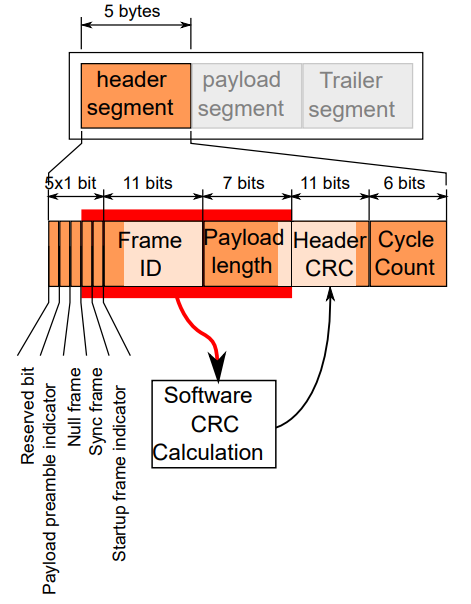
\includegraphics[width=1\textwidth]{capitoli/figure-protocolli/flexray-header.png}
        \caption{Struttura dell'header di un frame \emph{FlexRay}}
        \label{fig:flexray-header}
    \end{subfigure}
    \hfill
    \begin{subfigure}{0.4\textwidth}
        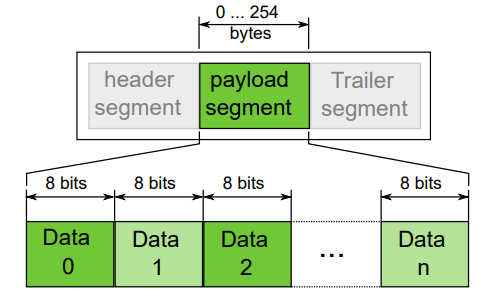
\includegraphics[width=1\textwidth]{capitoli/figure-protocolli/flexray-payload.png}
        \caption{Struttura del payload di un frame \emph{FlexRay}}
        \label{fig:flexray-payload}
    \end{subfigure}
    \centering
    \begin{subfigure}{0.4\textwidth}
        \vspace{0.3cm}
        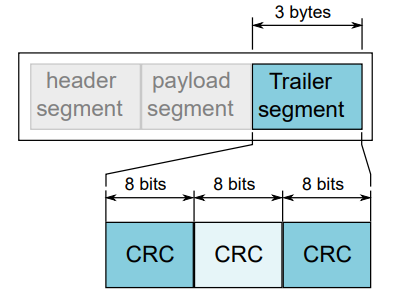
\includegraphics[width=1\textwidth]{capitoli/figure-protocolli/flexray-trailer.png}
        \caption{Struttura del trailer di un frame \emph{FlexRay}}
        \label{fig:flexray-trailer}
    \end{subfigure}
    \caption{Struttura di un frame \emph{FlexRay}}
    \label{fig:flexray-frame-structure}
\end{figure}

\begin{itemize}
    \item \textbf{Riservato}: 1 bit che è lasciato per sviluppi futuri;
    \item \textbf{Payload Preamble Indicator}:  1 bit che specifica se il campo \textbf{payload} è utilizzato per scambio di dati (bit impostato a $0$) oppure per un motivo diverso (bit impostato a $1$);
    \item \textbf{Null frame}: 1 bit che indica se il payload contiene dati validi (bit impostato a $1$) oppure se contiene dati non validi (bit impostato a $0$). In quest'ultimo caso, tutti i bit del campo \textbf{payload} vengono impostati a 0;
    \item \textbf{Sync Frame}: 1 bit che indica se il frame è di sincronizzazione (bit impostato a $1$) oppure no (bit impostato a $0$). I frame di sincronizzazione possono essere inviati solo se ci si trova in un segmento statico;
    \item \textbf{Startup Frame Indicator}: 1 bit che indica se il frame è di tipo \textbf{startup} (bit impostato a $1$) oppure no (bit impostato a $0$). I frame di startup sono dei tipi particolari di frame che possono essere inviati solo da nodi \emph{coldstart} per sfruttare il meccanismo dello \emph{startup} dei nodi, inoltre, questo tipo di frame dovrebbe avere sia questo bit sia il bit \textbf{sync} a $1$;
    \item \textbf{Frame ID}: 11 bit che definiscono lo slot temporale nel quale questo messaggio deve inviato. Ovviamente in un ciclo di comunicazione deve essere unico ed è un numero nel range 1-2047 (l'ID 0 non è valido);
    \item \textbf{Payload Length}: 7 bit che indicano quanti gruppi di 2 Byte sono presenti nel payload. Se ad esempio, questo campo viene impostato a 35, allora la lunghezza del payload sarà $35\times 2 = 70$ Byte.
    \item \textbf{Header CRC}: 11 bit che indicano il codice \textbf{CRC} per individuare errori nell'header. Viene calcolato tenendo in considerazione i bit \textbf{Sync frame}, \textbf{Startup Frame Indicator}, \textbf{Frame ID} e \textbf{Payload Length};
    \item \textbf{Cycle Count}: 6 bit che indicano in quale ciclo di comunicazione ci si trova al momento dell'invio del frame;
    \item \textbf{Payload}: segmento che ha una lunghezza massima di 254 Byte e che contiene i dati da inviare insieme al frame;
    \item \textbf{CRC}: 24 bit che rappresentato il codice \textbf{CRC} per individuare errori nel payload;
\end{itemize}

\subsection{Topologie supportate}
Il protocollo \emph{FlexRay} per come è stato progettato supporta diverse topologie di rete, in modo tale da adattarsi al meglio ad ogni tipo di situazione e garantire sempre elevati requisiti di affidabilità. Le topologie maggiormente utilizzate sono le seguenti:

\begin{figure}[h]
    \centering
    \begin{subfigure}{0.8\textwidth}
        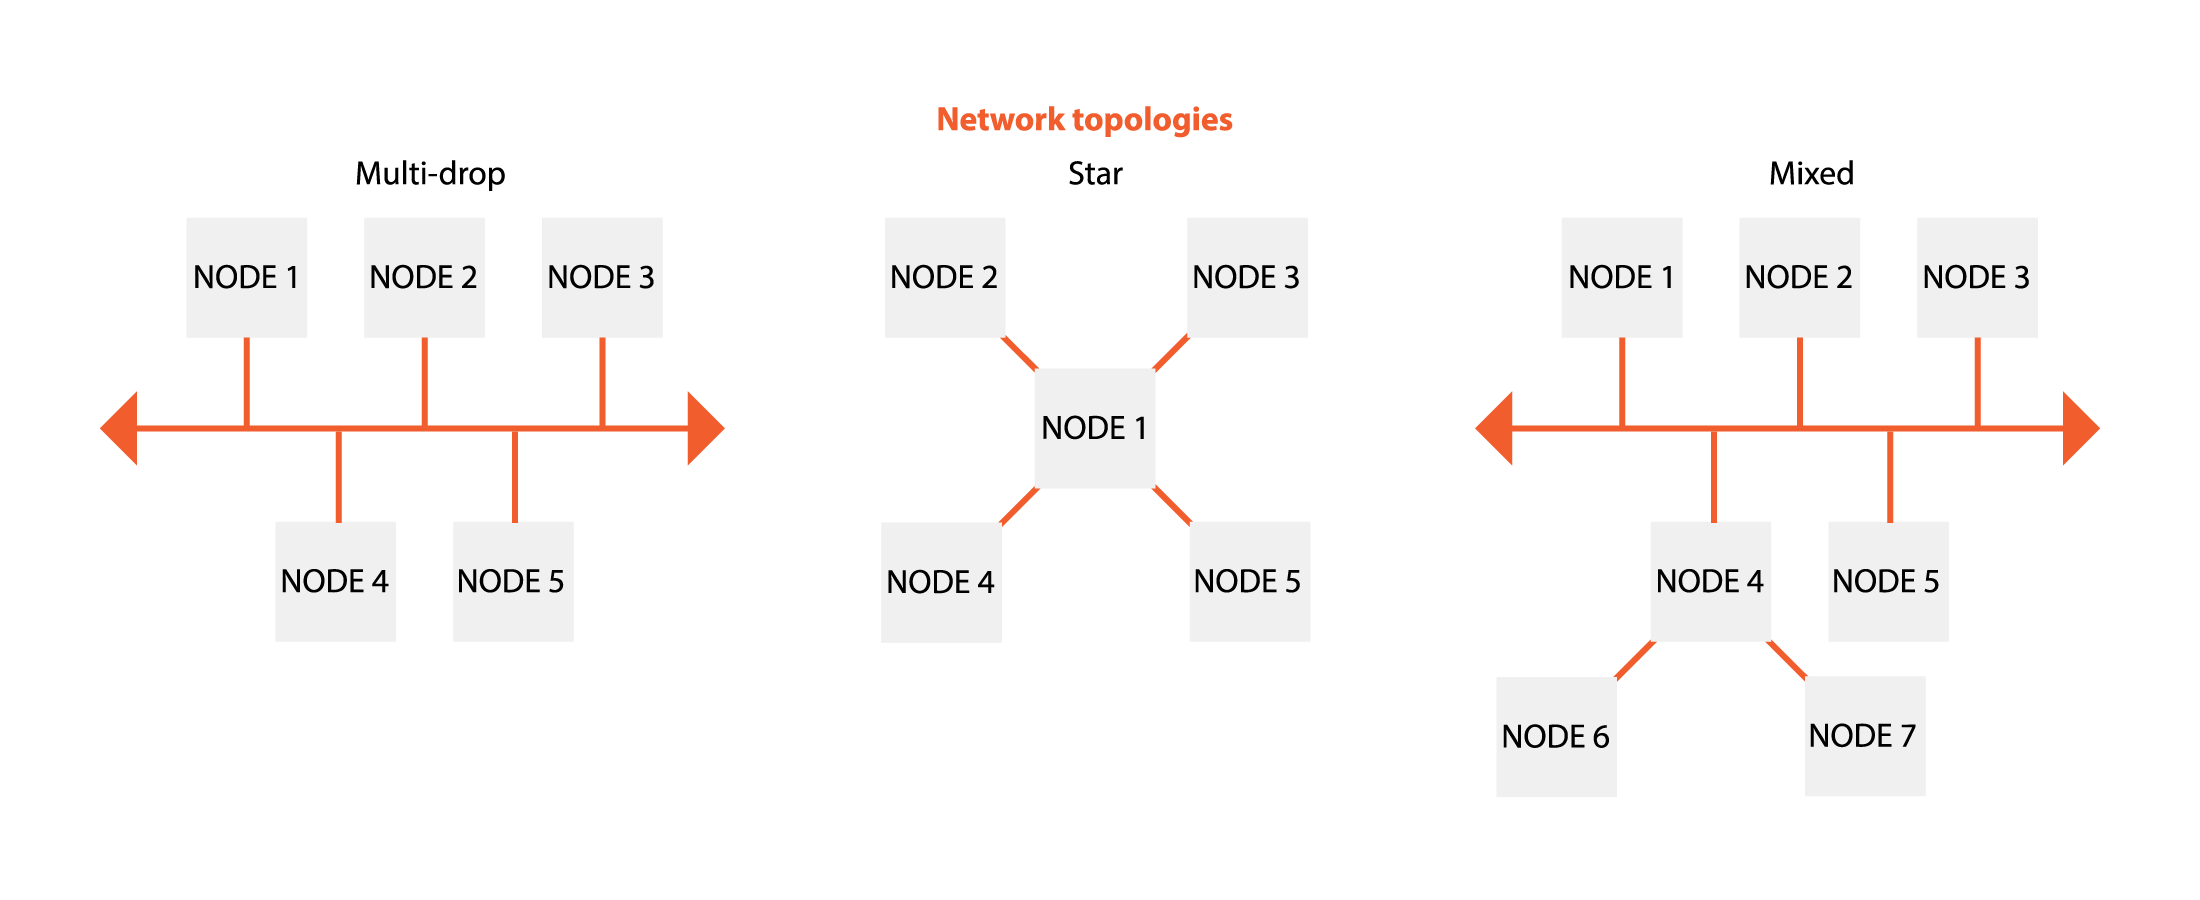
\includegraphics[width=1\textwidth]{capitoli/figure-protocolli/flexray-topologies.png}
        \caption{Topologie di rete a \emph{Bus}, \emph{Stella} e \emph{Ibrida}}
        \label{fig:flexray-topologies}
    \end{subfigure}
    \begin{subfigure}{0.5\textwidth}
        \vspace{0.3cm}
        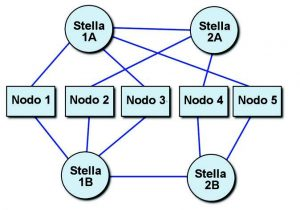
\includegraphics[width=1\textwidth]{capitoli/figure-protocolli/flexray-multiple-star.jpg}
        \caption{Topologia di rete a \emph{stella multipla}}
        \label{fig:flexray-multiple-star}
    \end{subfigure}
    \caption{Principali topologie di rete supportate da \emph{FlexRay}}
    \label{fig:flexray-supported-topologies}
\end{figure}

\begin{itemize}
    \item \textbf{Bus}: anche detta \emph{Multi-drop Bus} è la topologia più utilizzata (\autoref{fig:flexray-topologies}). In questo caso, c'è un cavo principale che fa da tronco (\emph{trunk}) e tutte le \emph{ECU} sono collegate a questo cavo tramite un connettore e un cavo più breve. Il cavo principale è poi terminato alle estremità con dei resistori per evitare problemi di \textbf{riflessione} del segnale. Questa è una delle topologie più utilizzate in quanto è anche quella utilizzata da \emph{CAN}, permettendo così una perfetta interoperabilità tra i due protocolli. Inoltre è anche la topologia che richiede un cablaggio più semplice rispetto alle altre topologie, rendendola la più economica. Tuttavia, essendo un unico cavo che collega tutti nodi, nel momento in cui questo si danneggia tutta la rete viene compromessa. Inoltre, essendo che questo cavo molto spesso è lungo, risente molto delle interferenze elettromagnetiche generate dal motore dell'automobile;
    \item \textbf{Stella}: in questa topologia (\autoref{fig:flexray-topologies}), tutte le \emph{ECU} sono collegate con una \emph{ECU} attiva che fa da \emph{centro-stella} e ha un funzionamento che è simile a quello di un \emph{hub} o uno \emph{switch} casalingo. Il vantaggio di questa topologia sta nel fatto che non c'è un unico cavo che collega tutti i nodi ma ci sono tanti piccoli segmenti che rendono i collegamenti indipendenti. Infatti, nel momento in cui un segmento si danneggia viene isolata solo una \emph{ECU} lasciando la restante rete completamente funzionante. Inoltre, avendo collegamenti più corti, nel momento in cui si collegano più centri-stella tra di loro è possibile raggiungere distanze maggiori senza risentire delle interferenze elettromagnetiche;
    \item \textbf{Ibrida}: topologia che combina i vantaggi della topologia a \emph{Stella} e della topologia \emph{Bus} (\autoref{fig:flexray-topologies}). In questo caso c'è un \emph{trunk} che collega sia singoli nodi che centri-stella, abbassando i costi dei cablaggi e sfruttando le performance e l'affidabilità delle stelle;
    \item \textbf{Stella multipla}: detta anche \textbf{Dual-channel single star} topologia che cerca di migliorare l'affidabilità della stella aggiungendo un'ulteriore stella che si collega a tutti i nodi o ad un sottoinsieme di nodi (\autoref{fig:flexray-multiple-star}). Questa topologia si può realizzare sfruttando il fatto che ogni cavo \emph{FlexRay} è composto da due fili, quindi un filo sarà collegato ad una stella mentre l'altro ad un'altra stella. Ovviamente questo tipo di topologia rende il cablaggio più complesso però migliora l'affidabilità complessiva della rete. Inoltre, è possibile anche collegare in cascata più stelle tra di loro realizzando una topologia \textbf{Dual-channel cascaded star} aggiungendo ulteriori collegamenti ridondanti. \cite{eos_flexray} \cite{flexray_specification}
\end{itemize}

\section{LIN}

\section{Confronto tra i tre protocolli}

\newpage
